\documentclass[aspectratio=169,11pt]{beamer}

\usepackage{booktabs}
\usepackage{graphicx}
\usepackage{array}
\usepackage{xcolor}
\usepackage{hyperref}

\usetheme{Madrid}
\usecolortheme{default}
\setbeamertemplate{navigation symbols}{}
\setbeamertemplate{footline}[frame number]
\graphicspath{{./}{../models/}}

\title[Image MMMD Testing]{Biomedical Image Two-Sample Testing with Learned Representations}
\subtitle{Representative experiments from the \texttt{yao/} workspace}
\author{Yao}
\institute{Biostatistics Project}
\date{2026-06-16}

\definecolor{mainblue}{RGB}{34, 88, 145}
\definecolor{accentred}{RGB}{180, 70, 55}
\definecolor{darkgreen}{RGB}{60, 130, 95}
\setbeamercolor{title}{fg=mainblue}
\setbeamercolor{frametitle}{fg=mainblue}
\setbeamercolor{structure}{fg=mainblue}

\newcommand{\good}[1]{\textcolor{darkgreen}{#1}}
\newcommand{\warn}[1]{\textcolor{accentred}{#1}}

\begin{document}

\begin{frame}
  \titlepage
\end{frame}

\begin{frame}{Research Question and Design}
  \begin{columns}[T,onlytextwidth]
    \begin{column}{0.48\textwidth}
      \textbf{Goal.} Test whether two image populations come from the same distribution.
      \vspace{0.5em}

      \textbf{Main questions}
      \begin{itemize}
        \item Which representation should be used: raw pixels, CLIP, DINOv2, or a trained CNN?
        \item Which testing layer should be used: the original MMMD test or lrj's stabilized variant?
        \item Can we obtain high power while controlling Type-I error?
      \end{itemize}
    \end{column}
    \begin{column}{0.48\textwidth}
      \textbf{Representative experiments}
      \begin{itemize}
        \item MNIST: small-image sanity check
        \item BloodMNIST-224: biomedical cell images with noise
        \item PathMNIST-28: comparison with dechao's CNN experiments
        \item NCT-CRC: pathology images, sample size, and lrj comparison
      \end{itemize}
    \end{column}
  \end{columns}
\end{frame}

\begin{frame}{Experimental Pipeline}
  \centering
  \begin{tabular}{>{\centering\arraybackslash}p{0.18\textwidth}
                  >{\centering\arraybackslash}p{0.24\textwidth}
                  >{\centering\arraybackslash}p{0.22\textwidth}
                  >{\centering\arraybackslash}p{0.18\textwidth}}
    \toprule
    Image data & Representation layer & Testing layer & Metrics \\
    \midrule
    MNIST \newline BloodMNIST \newline PathMNIST \newline NCT-CRC
    &
    Raw pixels \newline CLIP \newline DINOv2 \newline CNN features
    &
    GAUSS5 / GEXP-5 \newline NEW-MMMD
    &
    Power \newline Type-I error \newline sample-size curve \\
    \bottomrule
  \end{tabular}

  \vspace{1.3em}
  \begin{block}{Implementation choice}
    Images are first converted into reusable \texttt{embeddings.npy + metadata.csv} pools.
    Testing then repeatedly samples from these pools. Type-I experiments use matched null splits or shared-pool designs to avoid false-positive inflation.
  \end{block}
\end{frame}

\begin{frame}{MNIST: DINOv2 Degrades under Heavy Noise}
  \begin{columns}[T,onlytextwidth]
    \begin{column}{0.58\textwidth}
      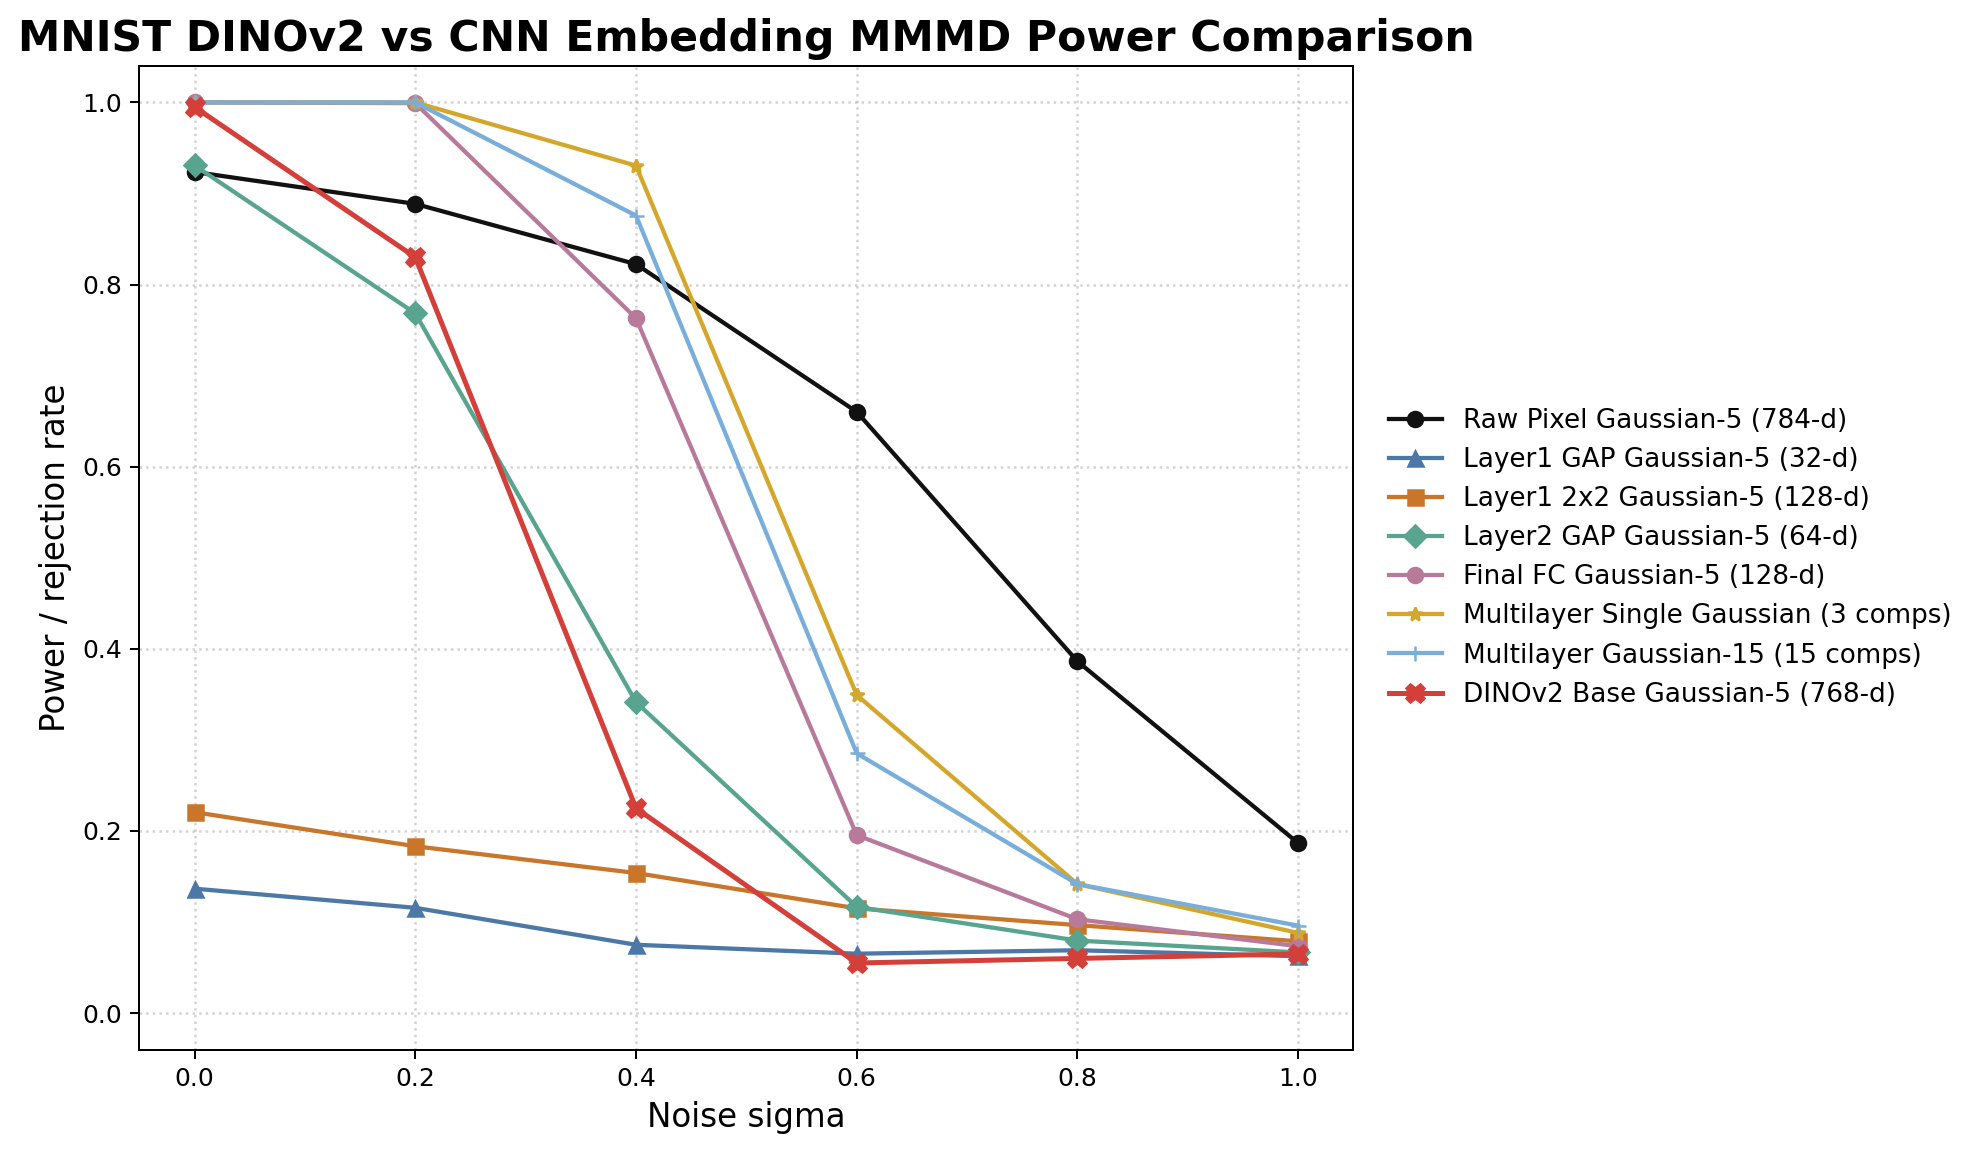
\includegraphics[width=\textwidth]{mnist_dinov2_dechao_power_medium/mnist_dinov2_vs_cnn_power_comparison.png}
    \end{column}
    \begin{column}{0.38\textwidth}
      \small
      \begin{tabular}{cc}
        \toprule
        $\sigma$ & DINOv2 power \\
        \midrule
        0.0 & 0.995 \\
        0.2 & 0.830 \\
        0.4 & 0.225 \\
        0.6 & 0.055 \\
        0.8 & 0.060 \\
        1.0 & 0.065 \\
        \bottomrule
      \end{tabular}
      \vspace{0.8em}

      \textbf{Interpretation.} MNIST images are $28\times28$ grayscale digits. DINOv2 requires resizing to a much larger input size, and the combination of resizing, interpolation, and Gaussian noise creates a strong domain mismatch.
    \end{column}
  \end{columns}
\end{frame}

\begin{frame}{BloodMNIST-224: CNN is the Most Robust Representation}
  \centering
  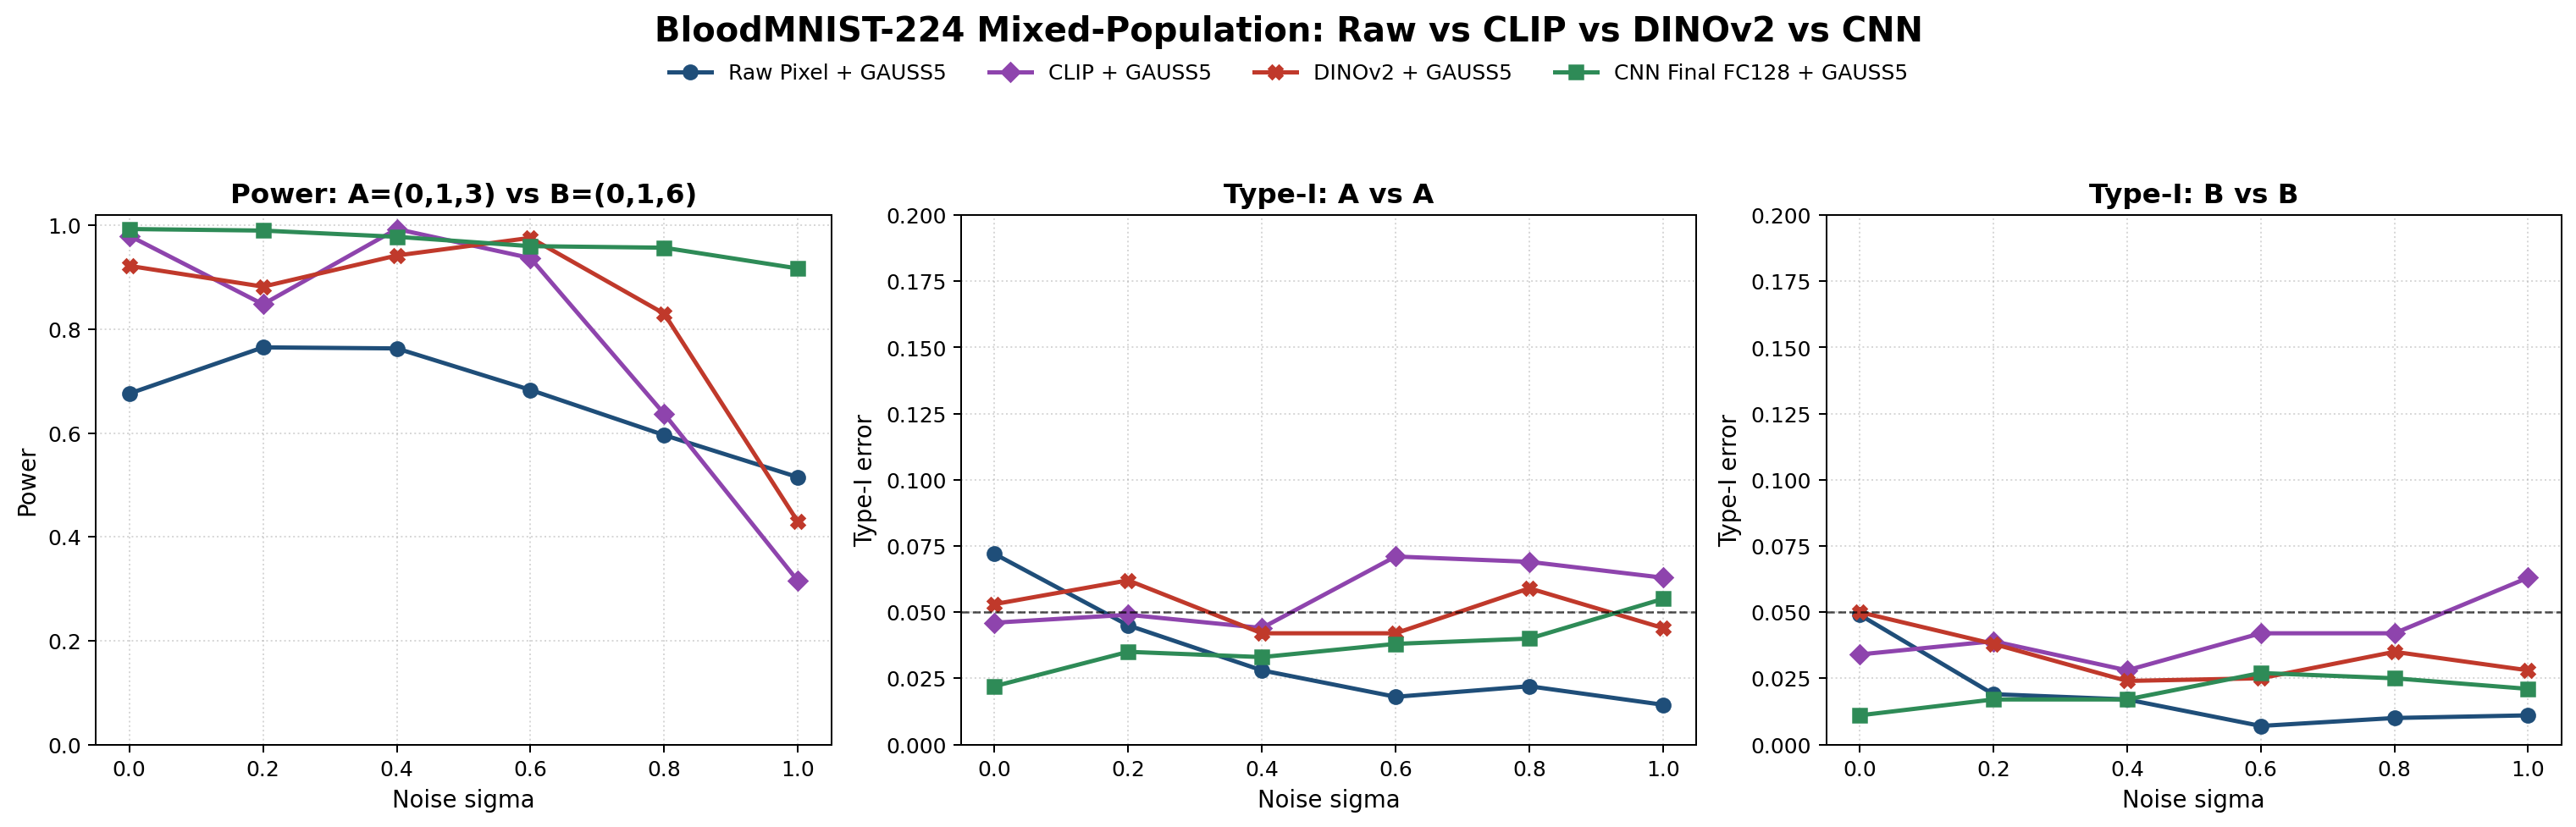
\includegraphics[width=0.72\textwidth]{bloodmnist224_mixed_raw_clip_dino_cnn_gauss5/bloodmnist_mixed_raw_clip_dino_cnn_gauss5.png}

  \vspace{-0.2em}
  \small
  \begin{tabular}{lccc}
    \toprule
    Method & Low-noise power & High-noise power & Type-I behavior \\
    \midrule
    Raw pixel + GAUSS5 & moderate & retains some signal & conservative \\
    CLIP + GAUSS5 & strong at low noise & drops at $\sigma=1.0$ & near nominal \\
    DINOv2 + GAUSS5 & strong at medium noise & better than CLIP & near nominal \\
    CNN final + GAUSS5 & \good{strongest overall} & \good{0.917 at $\sigma=1.0$} & slightly conservative \\
    \bottomrule
  \end{tabular}
\end{frame}

\begin{frame}{BloodMNIST-224: Learned Features Improve Sample Efficiency}
  \begin{columns}[T,onlytextwidth]
    \begin{column}{0.60\textwidth}
      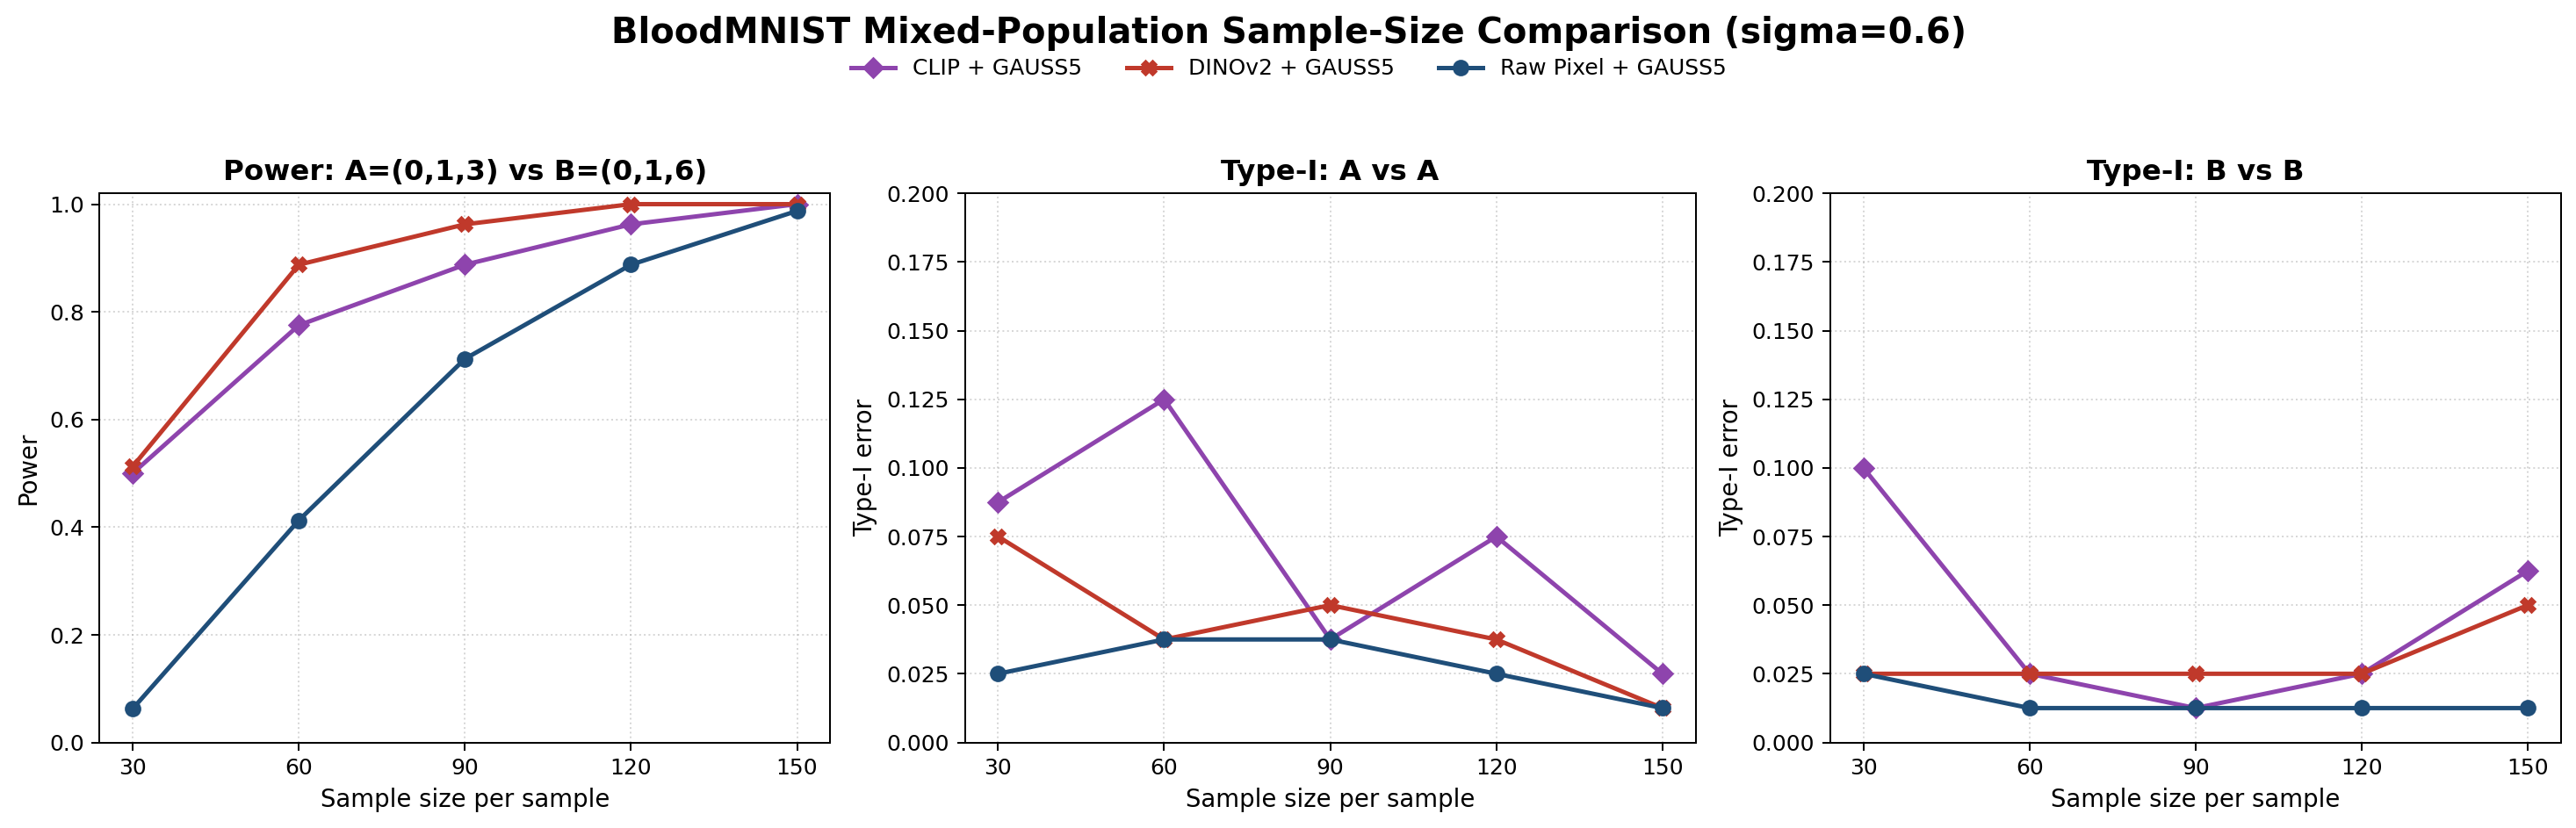
\includegraphics[width=\textwidth]{bloodmnist224_sample_size_sigma06/bloodmnist_mixed_sample_size_comparison.png}
    \end{column}
    \begin{column}{0.36\textwidth}
      \small
      Fixed noise level: $\sigma=0.6$.
      \vspace{0.5em}

      \begin{tabular}{cccc}
        \toprule
        $n$ & Raw & CLIP & DINOv2 \\
        \midrule
        30 & 0.063 & 0.500 & 0.513 \\
        60 & 0.413 & 0.775 & 0.888 \\
        90 & 0.713 & 0.888 & 0.963 \\
        120 & 0.888 & 0.963 & 1.000 \\
        150 & 0.988 & 1.000 & 1.000 \\
        \bottomrule
      \end{tabular}
      \vspace{0.8em}

      \textbf{Conclusion.} Learned embeddings greatly improve sample efficiency. Raw pixels need substantially larger samples to catch up.
    \end{column}
  \end{columns}
\end{frame}

\begin{frame}{PathMNIST-28: Alignment with Dechao's CNN Experiments}
  \begin{columns}[T,onlytextwidth]
    \begin{column}{0.58\textwidth}
      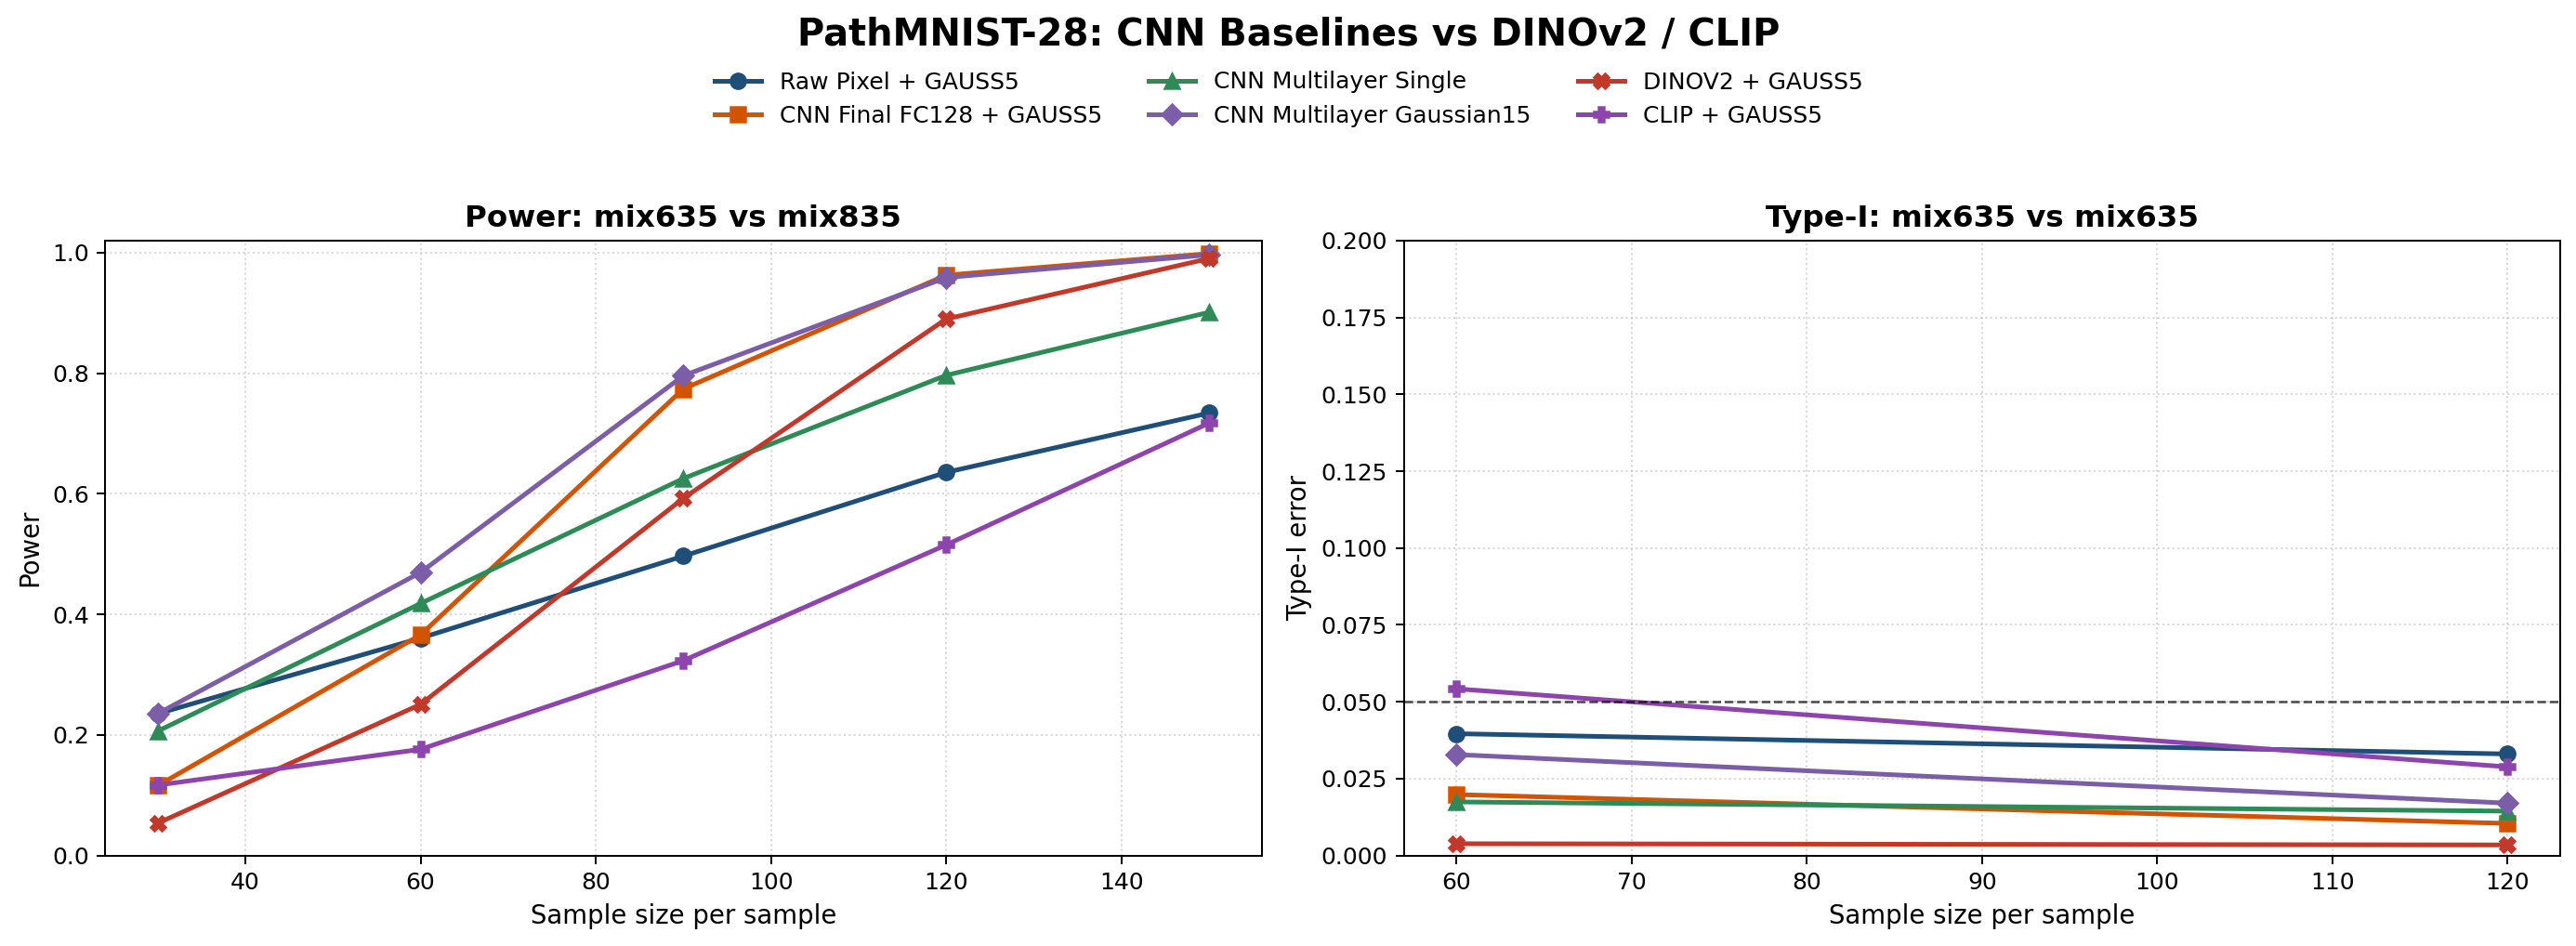
\includegraphics[width=\textwidth]{pathmnist28_vs_cnn_comparison/pathmnist_sample_size_vs_cnn.png}
    \end{column}
    \begin{column}{0.38\textwidth}
      \small
      \begin{tabular}{cccc}
        \toprule
        $n$ & CLIP & DINOv2 & Note \\
        \midrule
        30 & 0.117 & 0.053 & both weak \\
        60 & 0.176 & 0.251 & DINOv2 improves \\
        90 & 0.323 & 0.593 & gap increases \\
        120 & 0.515 & 0.890 & DINOv2 strong \\
        150 & 0.717 & 0.990 & near full power \\
        \bottomrule
      \end{tabular}
      \vspace{0.8em}

      \textbf{Conclusion.} DINOv2 becomes strong as sample size grows, but task-trained CNN baselines remain important in the small-to-medium sample regime.
    \end{column}
  \end{columns}
\end{frame}

\begin{frame}{NCT-CRC: Representation Comparison on Pathology Images}
  \begin{columns}[T,onlytextwidth]
    \begin{column}{0.60\textwidth}
      
\includegraphics[width=\textwidth]{nctcrc_sample_size_with_cnn/nctcrc_sample_size_comparison.png}
    \end{column}
    \begin{column}{0.36\textwidth}
      \small
      \begin{tabular}{ccccc}
        \toprule
        $n$ & Raw & CLIP & CNN & DINOv2 \\
        \midrule
        30 & 0.125 & 0.013 & 0.100 & 0.038 \\
        60 & 0.113 & 0.063 & 0.288 & 0.188 \\
        90 & 0.175 & 0.200 & 0.575 & 0.475 \\
        120 & 0.238 & 0.500 & 0.738 & 0.875 \\
        150 & 0.300 & 0.750 & 0.875 & 0.988 \\
        \bottomrule
      \end{tabular}
      \vspace{0.8em}

      \textbf{Conclusion.} CNN is stronger at small and medium sample sizes, while DINOv2 becomes the strongest representation at larger sample sizes.
    \end{column}
  \end{columns}
\end{frame}

\begin{frame}{lrj Method: More Stable, Often More Conservative}
  \centering
  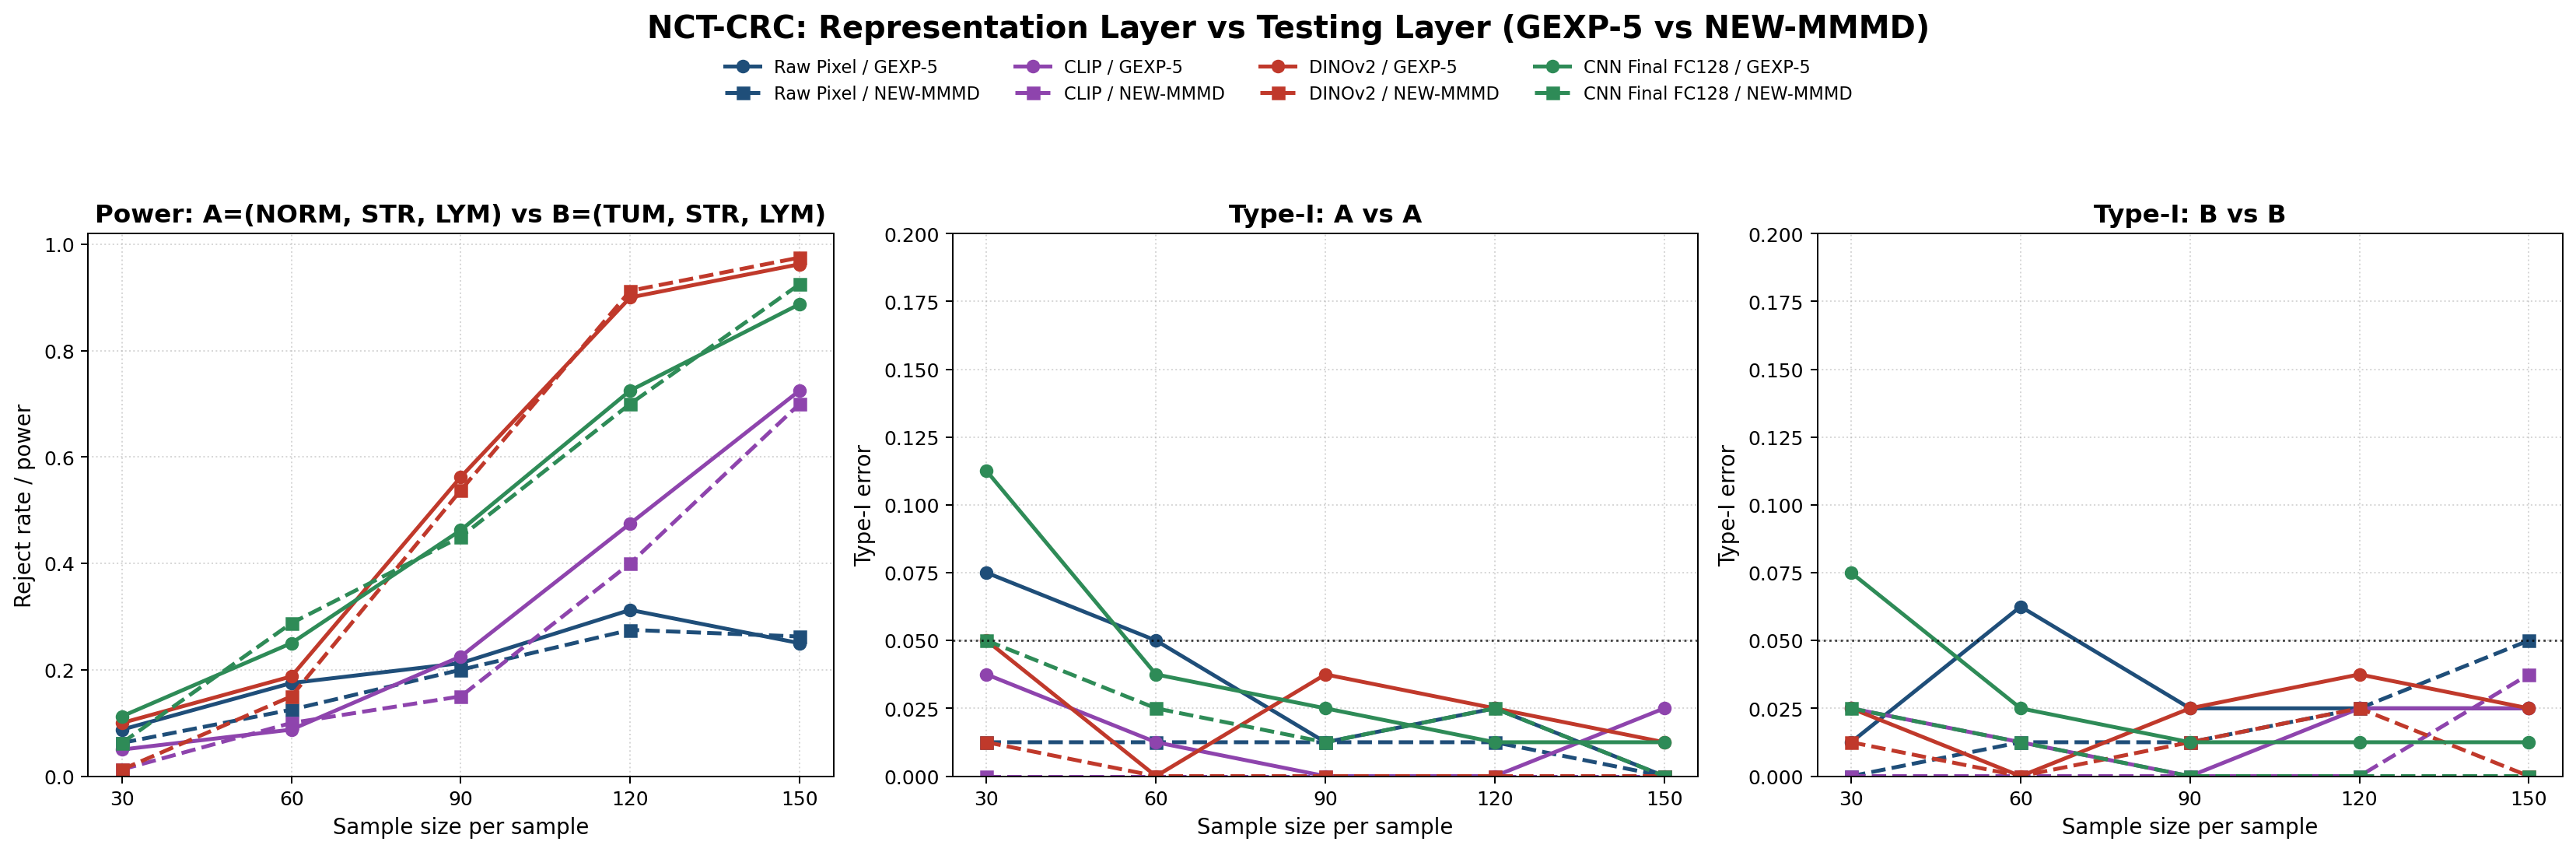
\includegraphics[width=0.76\textwidth]{nctcrc_lrj_all_representations/nctcrc_lrj_all_representations.png}

  \vspace{-0.2em}
  \small
  \begin{itemize}
    \item \textbf{GEXP-5:} original multi-kernel MMMD-style testing layer; often has higher small-sample power.
    \item \textbf{NEW-MMMD:} lrj's covariance-stabilized variant with kernel pruning; often lowers Type-I error.
    \item At $n=150$, NEW-MMMD matches or slightly exceeds GEXP-5 for DINOv2 and CNN features, but it can lose power in small samples.
  \end{itemize}
\end{frame}

\begin{frame}{Takeaways}
  \begin{block}{Main findings}
    \begin{itemize}
      \item The representation layer is the dominant factor: raw pixels, CLIP, DINOv2, and CNN features lead to very different testing power.
      \item On BloodMNIST-224, the task-trained CNN is the most robust representation under Gaussian noise.
      \item On NCT-CRC, DINOv2 overtakes the CNN at large sample sizes, while the CNN is more competitive at smaller sample sizes.
      \item CLIP is usually weaker than DINOv2 for these morphology-driven biomedical tasks.
      \item lrj's NEW-MMMD is best viewed as a stabilization and Type-I-control improvement, not a guaranteed power booster.
    \end{itemize}
  \end{block}

  \begin{block}{Next steps}
    Increase Monte Carlo repeats, run NEW-MMMD on BloodMNIST, add stain/color perturbations, and compare with stronger biomedical encoders.
  \end{block}
\end{frame}

\end{document}
